\iffalse
\documentclass[journal,12pt,twocolumn]{IEEEtran}
\usepackage{cite}
\usepackage{amsmath,amssymb,amsfonts,amsthm,mathtools}
\usepackage{algorithmic}
\usepackage{graphicx}
\parindent 0px
\bibliographystyle{IEEEtran}
\title{GATE 2023-EE Q49}
\author{EE23BTECH11052 - Abhilash Rapolu}
\begin{document}
\maketitle
\newpage
\textbf{Question 49}: The period of the discrete-time signal x[n] described by the equation below is N =\ (Round off to the nearest integer).
$$x[n] = 1 + 3\sin\left(\frac{15\pi}{8}n + \frac{3\pi}{4}\right) - 5\sin\left(\frac{\pi}{3}n - \frac{\pi}{4}\right)$$
\textbf{Solution:}
\fi
\begin{table}[htbp]
\centering
\begin{tabular}{|l|l|c|}
\hline
\textbf{Parameter} & \textbf{Description} & \textbf{Value} \\
\hline
$f_{1}$ & Sinusoid1 Frequency & 15/16 \\
\hline
$f_{2}$ & Sinusoid2 Frequency & 6 \\
\hline
\end{tabular}

 
\caption{Given parameters list}
\end{table}

The time period must be an integer for a discrete-time signal.
\begin{align}
T_1 &= \frac{1}{f_1} = \frac{16}{15} \\
T_2 &= \frac{1}{f_2} = 6 \\
N &= \text{LCM}(T_1, T_2) = 48
\end{align}

The Time Period of the signal is \(N = 48\).

Let's find the Discrete Fourier Transform (\(X[k]\)):
\begin{align}
X[k] &= \sum_{n=0}^{N-1} x[n]e^{-j\frac{2\pi}{N}kn} \\
X[k] &= \sum_{n=0}^{47} \left(1 + 3\sin\left(\frac{15\pi}{8}n + \frac{3\pi}{4}\right) 
- 5\sin\left(\frac{\pi}{3}n - \frac{\pi}{4}\right)\right) \cdot e^{-j\frac{2\pi}{48}kn} \\
X[k] &= \begin{cases}
    48 & \text{if } k = 0 \\
    50.9117 - 50.9117j & \text{if } k = 3 \\
    0 & \text{otherwise}
\end{cases}
\end{align}

\begin{figure}[!ht] 
\centering
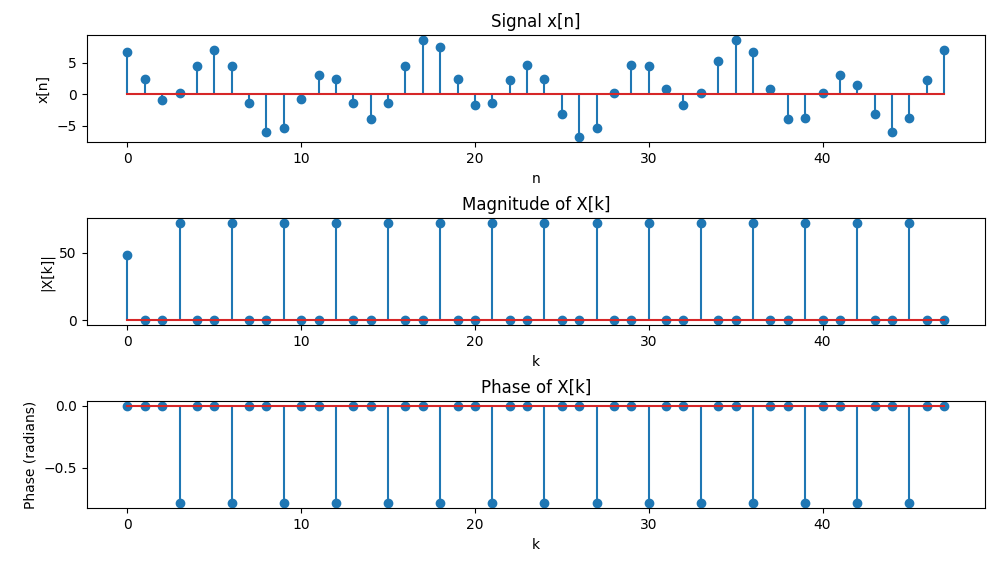
\includegraphics[width=\columnwidth]{2023/EE/49/figs/EE.49.png}
\end{figure}

%\end{document}









